%D�finir le format du document: papier, taille de police, type de document, etc.
\documentclass[a4paper, 11pt]{article}

%%%%%%%%% Packages externes utilis�s %%%%%%%%%%%%%%%%%%%
\usepackage[french]{babel}
\usepackage[latin1]{inputenc}
\usepackage[T1]{fontenc}
\usepackage{verbatim}
\usepackage{graphicx}
\usepackage{epstopdf}
\usepackage{macro}
\usepackage{algorithm}
\usepackage{algorithmic}


%La mise en page du rapport, NE PAS MODIFIER.
\usepackage{geometry}
 \geometry{
 a4paper,
 left=20mm,
 right=20mm,
 top=20mm,
 bottom=20mm,
 }

%%%%%%%%% Le corps du document entre begin et end %%%%%%%%%%%%%%%%%%%
\begin{document}

%Page de garde
%%%%%%%%%%%%%%% Page de garde %%%%%%%%%%%%%%%%%%%

\begin{titlepage}{
    \begin{center}
				\noreffig{images/UCP_logo.jpg}{5cm}{3.5cm}
        \skip {0}
        {\Large \textbf {Universit� de Cergy-Pontoise}} \\
        \vspace* {10mm}
        {\Large \textbf {Rapport de Projet}} \\
        \vspace* {10mm}
        pour l'Unit� d'Enseignement "G�nie Logiciel et Programmation" \\
        \textbf {Licence d'Informatique 2e Ann�e} \\
        \vspace* {10mm}

	sur le sujet \\
        \vspace* {10mm}
	{\Huge \textbf{Histoire}} \\
        \vspace* {10mm}
 	r�dig� par \\
        \vspace* {10mm}
        {\Large \textbf {Matteo STAIANO, Mathieu HANNOUN}} \\
				\vspace* {10mm}
				\noreffig{images/histoire.jpg}{13cm}{7cm} \\
        \date Mai 2017
        \vspace* {10mm}
	\end{center}
}
\end{titlepage}


%G�n�ration automatique de la table des mati�res, de la liste des figures et de la liste des tableaux
\tableofcontents
\listoffigures
\listoftables

%Une section "remerciements" pourrait �tre int�ressante. C'est une section non num�rot� (avec un * )
\section*{Remerciements}
Les auteurs du projet voudraient remercier...
\newpage
\section{Pr�sentation du projet}
\label{sec:presentation}

\subsection{Contexte}
Le module de G�nie Logiciel et Programmation de L2 nous demandant la r�alisation d'un projet en Java et souhaitant repr�senter un syst�me et son �volution suivant diff�rents stimulis, al�atoires ou non, il paraissait judicieux de s'orienter vers un sujet de ce type.
Ayant initialement choisi Psychologie et le projet �tant d�j� attribu� � un autre groupe, le choix d'histoire parut logique.
\subsection{Objet}
Repr�senter sous la forme d'un journal agr�ment� d'objets graphiques l'�volution d'un nombre limit� de peuples au cours du temps et en fonction d'un certain nombre d'�v�nements, al�atoires ou non.
\subsection{Organisation}
\begin{itemize}
\bulletitem Matteo Staiano : Interface Graphique
\bulletitem Mathieu Hannoun : Conception backend
\bulletitem Commun : R�flexion algorithmique, debugging, compte-rendus et �l�ments de livraison finale.
\end{itemize}
\subsection{Environnements de travail et outils utilis�s}
\begin{itemize}
\bulletitem Programmation Java : Eclipse, Intellij IDEA
\bulletitem VCS : GitHub
\bulletitem Production du rapport \LaTeX{} : TeXnicCenter
\end{itemize}
\section{Sp�cifications et fonctionnalit�s finales}
\label{sec:specifications}

\subsection{Backend}
\paragraph{Peuple}
Chaque peuple commence avec des attributs principaux bien sp�cifiques dont d�coulent des attributs secondaires.
\subparagraph{Attributs principaux\protect\footnote{D�tails des relations entre attributs dans le sch�ma en derni�re page}}
\begin{itemize}
\bulletitem Ressources
\bulletitem Population
\bulletitem Agressivit�
\bulletitem Education
\bulletitem Territoire
\end{itemize}
\subparagraph{Attributs secondaires}
\begin{itemize}
\bulletitem A
\bulletitem B
\bulletitem C
\end{itemize}
\smallbreak
Les diff�rents peuples peuvent avoir des relations avec les autres sous deux formes : la guerre et le commerce. Le d�clenchement de ces relations ne d�pend que des diff�rents attributs secondaires.
\paragraph{Guerre et commerce}
Chaque tour, des guerres et des liens commerciaux commencent, ou non, entre les peuples, en fonction de leurs caract�ristiques secondaires. Ces relations n'influent que sur les attributs principaux.
\newline
La guerre est co�teuse en population pour les deux peuples, mais apporte richesse et territoire au peuple disposant de la plus grande puissance militaire.
\newline
Le commerce apporte un b�n�fice mutuel aux deux peuples, mais plus un peuple dispose de puissance politique et plus il sera capable de tirer b�n�fice d'un commerce avec un autre.
\clearpage
\section{Interface Utilisateur}
\label{sec:gui}

\subsection{Fen�tre}
La fen�tre du programme aura une taille pr�d�finie de 1280x720 pixels et n'est pas redimensionnable. Cette dimension a �t� choisir car elle correspond � une r�solution de 16:9 et est � la fois suffisamment petite pour ne pas d�border de la plupart des �crans, et suffisamment grande pour nous permettre d'afficher des �l�ments suffisamment d�taill�s.
\begin{figure}[H]
	\centering
		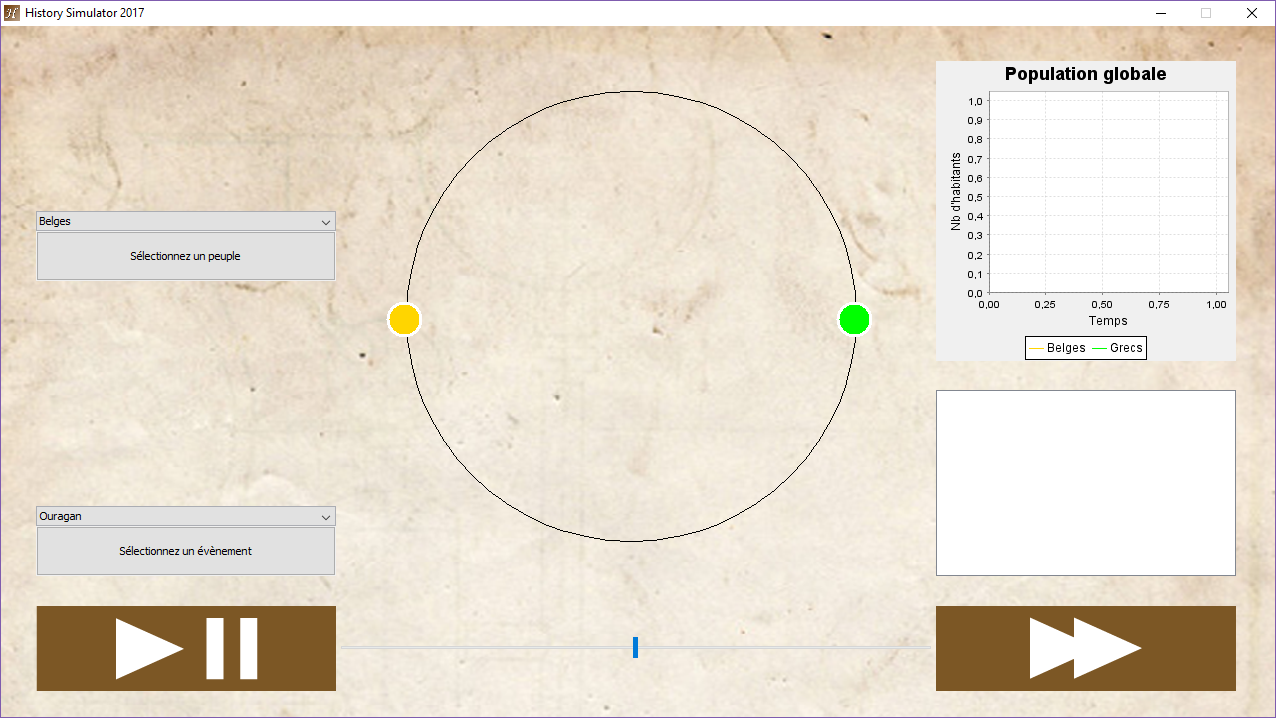
\includegraphics[scale=0.5]{images/window.png}
	\caption{Fen�tre}
	\label{fig:window}
\end{figure}

\subsection{�coulement du temps}
Dans la partie basse de l'interface, trois �l�ments permettent de g�rer le passage du temps. � gauche, un bouton permet de mettre en pause ou de reprendre le passage automatique des cycles. Au milieu, un curseur sert � r�gler la vitesse d'�coulement du temps lors des cycles automatiques. 
\newline
Enfin, � droite, un bouton permet de passer au cycle suivant manuellement, m�me si l'�coulement du temps est en pause.

\subsection{Statistiques centrales}
Au centre de la fen�tre, des statistiques sont affich�es. Par d�faut, il s'agira d'un diagramme repr�sentant les pays ainsi que leurs relations. Si un peuple est s�lectionn�\footnote{Voir plus bas pour la s�lection d'un peuple}, les statistiques affich�es seront celles du peuple en question, et plus de d�tails seront fournis sur celui-ci.
\begin{figure}[H]
	\centering
		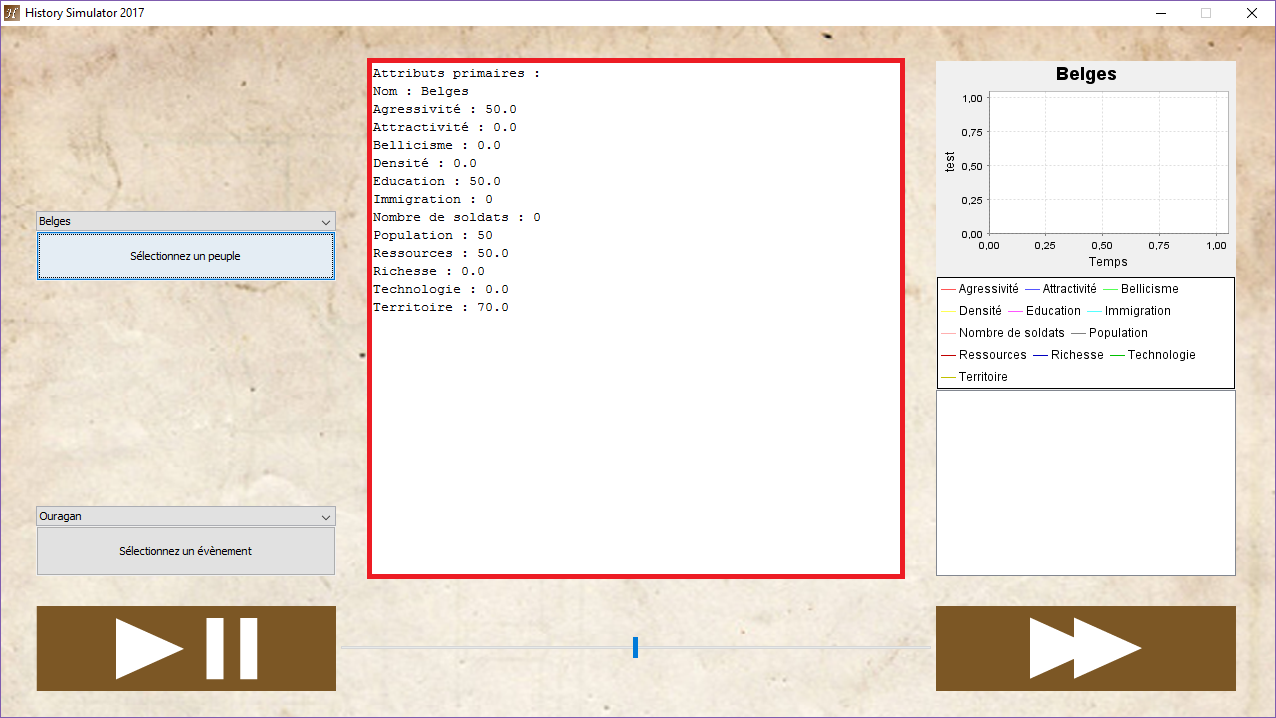
\includegraphics[scale=0.5]{images/details.png}
	\caption{D�tails}
	\label{fig:details}
\end{figure}

\subsection{S�lectionner un peuple}
Un menu d�roulant comportant tous les peuples et un bouton de validation sont � gauche de la fen�tre. Ceux-ci permettent de s�lectionner un peuple. En validant, on a acc�s � ses statistiques d�taill�es au centre de l'interface.
\newline
Il y a �galement une option \textit{Aucun} permettant de revenir � l'affichage des statistiques globales des relations entre les peuples.

\subsection{S�lectionner un �v�nement}
Les �v�nements peuvent �tre d�clench�s manuellement par l'utilisateur, via un menu d�roulant et un bouton de validation. Il est �galement possible de param�trer la puissance de l'�v�nement, ainsi que de d�sactiver les �v�nements al�atoires.
\newline
Si un peuple est s�lectionn�, l'�v�nement le concernera. Sinon, le menu d�roulant n'affichera que les �v�nements d'ampleur globale.
\subsection{Compte-rendu des �v�nements}
� droite de l'interface, une zone de texte liste tous les �v�nements s'�tant produits au cours du dernier cycle.
%\clearpage
\section{Conclusion}
\label{sec:conclusion}

\noindent Au terme de ce projet, nous avons beaucoup appris et sommes fiers du programme final.
\newline
N�anmoins, celui-ci est loin d'�tre parfait, et plusieurs am�liorations seraient encore possibles.
\newline
Il serait par exemple possible de permettre � l'utilisateur de cr�er lui-m�me les peuples qu'il souhaite voir en jeu, ou le th�me qu'il souhaite utiliser.
\newline
L'�quilibrage n'est lui non plus pas parfait, et il serait int�ressant de cr�er un syst�me d'�quilibrage automatique en fonction des r�sultats des derni�res simulations.
\newline
\newline
Toutefois, nous sommes parvenus � nous organiser correctement de mani�re � ce que l'interface utilisateur et le moteur avancent de mani�re parall�le et synchronis�e. Les objectifs ont �t� r�alis�s dans les d�lais que nous avions convenu et nous avons tous deux consolid� nos connaissances g�n�rales et nos m�thodes de travail.

%R�f�rences bibliographiques du document
\bibliographystyle{plain}
\bibliography{bibliographies}
\nocite{*}

\end{document}
